\documentclass[final,hyperref={pdfpagelabels=false}]{beamer}
\usepackage{grffile}
\mode<presentation>{\usetheme{I6pd2}}
\usepackage[english]{babel}
\usepackage[latin1]{inputenc}
\usepackage{amsmath,amsthm, amssymb, latexsym}
%\usepackage{times}\usefonttheme{professionalfonts}  % obsolete
%\usefonttheme[onlymath]{serif}
\boldmath
\usepackage[orientation=portrait,size=a0,scale=1.4,debug]{beamerposter}
% change list indention level
% \setdefaultleftmargin{3em}{}{}{}{}{}


%\usepackage{snapshot} % will write a .dep file with all dependencies, allows for easy bundling

\usepackage{array,booktabs,tabularx}
\newcolumntype{Z}{>{\centering\arraybackslash}X} % centered tabularx columns
\newcommand{\pphantom}{\textcolor{ta3aluminium}} % phantom introduces a vertical space in p formatted table columns??!!

\listfiles

%%%%%%%%%%%%%%%%%%%%%%%%%%%%%%%%%%%%%%%%%%%%%%%%%%%%%%%%%%%%%%%%%%%%%%%%%%%%%%%%%%%%%%
\graphicspath{{figures/}}

\setlogo{logos/w3-simple}
\setauthorurl{Jeffrey Burdges}
\setauthoremail{jeff@web3.foundation}

\title{\huge Assessing or incentivising correct mixing without authorities}
\author{Jeffrey Burdges}
\institute[Web 3 Foundation]{Web 3.0 Foundation}
\date[Feb 2020]{Feb 2020}

%%%%%%%%%%%%%%%%%%%%%%%%%%%%%%%%%%%%%%%%%%%%%%%%%%%%%%%%%%%%%%%%%%%%%%%%%%%%%%%%%%%%%%
\newlength{\columnheight}
\setlength{\columnheight}{105cm}


%%%%%%%%%%%%%%%%%%%%%%%%%%%%%%%%%%%%%%%%%%%%%%%%%%%%%%%%%%%%%%%%%%%%%%%%%%%%%%%%%%%%%%
\begin{document}
\begin{frame}
  \begin{columns}
    % ---------------------------------------------------------%
    % Set up a column 
    \begin{column}{.49\textwidth}
      \begin{beamercolorbox}[center,wd=\textwidth]{postercolumn}
        \begin{minipage}[T]{.95\textwidth}  % tweaks the width, makes a new \textwidth
          \parbox[t][\columnheight]{\textwidth}{ % must be some better way to set the the height, width and textwidth simultaneously
            % Since all columns are the same length, it is all nice and tidy.  You have to get the height empirically
            % ---------------------------------------------------------%
            % fill each column with content            
            \begin{block}{Assessment problem}
                Anonymity systems {\em assess} routers for performance, capacity, and reliability, \\ % \hspace*{3pt} 
                but do so using centralised infrastructure.  Can one decentralize assessment? \\ \smallskip
                
                Example: Tor's bandwidth authority and special role flags \\ \smallskip
            \end{block}
            \vfill
            \begin{block}{Rewards problem}
                Can one ``pay'' relays securely and efficiently? And avoid billing users?
            \end{block}
            \vfill
            \begin{block}{Bootstrap problem}
                % Proof-of-work coins only pay hydroelectric owners in China, but
                % proof-of-stake coins only pay people listed in the geneis block.
                Can proof-of-stake cybercoins pay unstaked node operators?
            \end{block}
            \vskip1ex
            \vfill
            \begin{block}{Mix networks} % {Metadata protection}
                \hspace*{5pt} {\it ``[Tor does not] protect against an attacker who can see .. both \\
                \hspace*{5pt} traffic going into [and] coming out of the Tor network .. as \\
                \hspace*{5pt} simple statistics let you decide whether [both flows] match up.''} \\
                \hspace*{30pt} \normalfont --Roger Dingledine, ``One cell is enough ..'' 
                \begin{columns}
                \begin{column}{.64\textwidth}
                Among the few known ``anonymous'' messaging strategies, non-verifiable mix networks provide the least expensive and most scalable alternative, but..
                \end{column}
                \begin{column}{.34\textwidth}
                \begin{center}
                
\includegraphics[width=0.75\textwidth]{../talks/pics/mix/initial} % was width=0.85
                \end{center}
                \end{column}
                \end{columns}                
                \begin{itemize}
                \item 
                Mixnets incur latency due to a mixing strategy (Poison or Stop-and-Go). \\
                We cannot adapt legacy protocols like HTTP to this higher latency, but.. \\
                we can design new protocols around the higher latency.
                \item 
                Mixnets require cover traffic (see Anonymity Trilemma \cite{anonymity_trilemma}) % \\
                \end{itemize}
            \end{block}
            \vfill
            \begin{block}{Cover loops}
                We've blend several cover categories using memoryless property of
                geometric or exponential distributions, several go nowhere special, but.. \\ \smallskip

                Users maintain incoming cover traffic by sending themselves loop messages. % , which \\ hides their real incoming messages.

                In Loopix \cite{Loopix}, mix nodes send themselves loop cover traffic too, which \\
                \begin{itemize}
                \item reduces adversaries' gains from monitoring mixes \cite[\S4.1.3: Thm 1 vs 2]{Loopix}, % and % see Theorem 1 vs 2 in \S4.1.3 of \cite{Loopix}.
                \item enable defenses against active attacks like n-1 attacks \cite[\S4.2.1]{Loopix}.
                \end{itemize}

                \begin{center}
                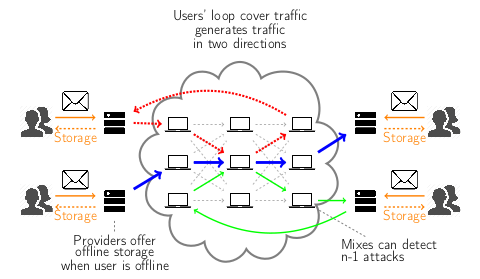
\includegraphics[trim=0 0 0 50,clip,width=\textwidth]{../talks/pics/loopix/achitecture}
                \end{center}

            \end{block}
            \vfill
			\begin{myblock}{References}
				\footnotesize
				\bibliographystyle{abbrv}
				\bibliography{../mix}
			\end{myblock}\vfill
          }
        \end{minipage}
      \end{beamercolorbox}
    \end{column}
    % ---------------------------------------------------------%
    % end the column

    % ---------------------------------------------------------%
    % Set up a column 
    \begin{column}{.49\textwidth}
      \begin{beamercolorbox}[center,wd=\textwidth]{postercolumn}
        \begin{minipage}[T]{.95\textwidth} % tweaks the width, makes a new \textwidth
          \parbox[t][\columnheight]{\textwidth}{ % must be some better way to set the the height, width and textwidth simultaneously
            % Since all columns are the same length, it is all nice and tidy.  You have to get the height empirically
            % ---------------------------------------------------------%
            % fill each column with content

            \begin{block}{Assumptions}
              \begin{itemize}
              \item Some mix nodes have stake in some limited resource, but not all, and
              non-transferable resources work, ala proof-of-personhood.
              \item 
              \end{itemize}
            \end{block}
            \vfill

            \begin{block}{Databases}
              \begin{columns}
                \begin{column}{.6\textwidth}
                  \begin{itemize}
                  \item AR-Face 
                    \begin{itemize}
                    \item variations in illumination
                    \item many different facial expressions
                    \end{itemize}
                  \item CMU-PIE
                    \begin{itemize}
                    \item variations in illumination (frontal images from the illumination subset)
                    \end{itemize}
                  \end{itemize}
                \end{column}
                \begin{column}{.39\textwidth}
                  \includegraphics[width=0.22\linewidth]{hanselmann-databases/arface/train/png/occlusions/arneutral/m-016-1}
                  \-
                  \includegraphics[width=0.22\linewidth]{hanselmann-databases/arface/train/png/cropped/m-016-4}
                  \-
                  \includegraphics[width=0.22\linewidth]{hanselmann-databases/arface/test/png/occlusions/ar1sun/m-016-8}
                  \-
                  \includegraphics[width=0.22\linewidth]{hanselmann-databases/arface/test/png/occlusions/ar1scarf/m-016-11}
                  \vskip3ex

                  \includegraphics[width=0.22\linewidth]{hanselmann-databases/cmupie/test/png/cropped/00-27-02}
                  \-
                  \includegraphics[width=0.22\linewidth]{hanselmann-databases/cmupie/test/png/cropped/00-27-17}
                  \-
                  \includegraphics[width=0.22\linewidth]{hanselmann-databases/cmupie/test/png/cropped/00-27-18}
                  \-
                  \includegraphics[width=0.22\linewidth]{hanselmann-databases/cmupie/test/png/cropped/00-27-20}
                \end{column}
              \end{columns}
            \end{block}
            \vfill
            \begin{block}{Results: Manually Aligned Faces}
              \begin{itemize}
              \item AR-Face: 110 classes, 770 train, 770 test
              \end{itemize}
              \vskip-0.5ex
              \begin{table}
                \centering
                \small
                \begin{tabular}{@{} p{.2\linewidth} p{.18\linewidth} p{.25\linewidth} r r r @{}}
                  \toprule 
                  Descriptor &  Extraction        & \multicolumn{1}{p{.2\linewidth}}{\# Features}           & \multicolumn{3}{c @{}}{Error Rates [\%]}         \\
                  \cmidrule(l){4-6}
                             &                    &                                                      & \multicolumn{1}{c}{Maximum} & \multicolumn{1}{c}{Grid} & \multicolumn{1}{c @{}}{Grid-Best} \\
                  \cmidrule(r){1-1}  \cmidrule(lr){2-2}   \cmidrule(lr){3-3}                               \cmidrule(lr){4-4}            \cmidrule(lr){5-5}         \cmidrule(l){6-6}  
                  SURF-64    & IPs                & \pphantom{1}64 $\times$ 5.6 (avg.)                    & 80.64     &  84.15  & 84.15     \\
                  SIFT       & IPs                & 128 $\times$ 633.78 (avg.)                           & 1.03      &  95.84  & 95.84      \\
                  \addlinespace
                  SURF-64    & 64x64-2 grid       & \pphantom{1}64 $\times$ 1024                          & 0.90      &  0.51   & 0.90      \\  
                  SURF-128   & 64x64-2 grid       & 128 $\times$ 1024                                    & 0.90      &  0.51   & 0.38       \\
                  SIFT       & 64x64-2 grid       & 128 $\times$ 1024                                    & 11.03     &  0.90   & 0.64       \\
                  \addlinespace
                  U-SURF-64  & 64x64-2 grid       & \pphantom{1}64 $\times$ 1024                          & 0.90      &  1.03   & 0.64      \\ 
                  U-SURF-128 & 64x64-2 grid       & 128 $\times$ 1024                                    & 1.55      &  1.29   & 1.03       \\ 
                  U-SIFT     & 64x64-2 grid       & 128 $\times$ 1024                                    & \textbf{0.25}  &  \textbf{0.25}   & \textbf{0.25}  \\
                  % \midrule
                  % \multicolumn{3}{l}{Modular PCA \cite{TanChen:subpatternPCA:Neurocomputing2005}}                         & 14.14 \\
                  % \multicolumn{3}{l}{Adaptively weighted Sub-Pattern PCA \cite{TanChen:subpatternPCA:Neurocomputing2005}} & 6.43  \\
                  % \multicolumn{3}{l}{DCT \cite{ekenel:LocalapFaceRecog:cvprbw2006}}                                       & 4.70  \\
                  \bottomrule
                \end{tabular}
              \end{table}

              \vskip1ex
              \begin{itemize}
              \item CMU-PIE: 68 classes, 68 train (``one-shot'' training), 1360 test
              \end{itemize}
              \vskip-0.5ex
              \begin{table}
                \centering
                \small
                \begin{tabular}{@{} p{.2\linewidth} p{.18\linewidth} p{.25\linewidth} r r r @{}}
                  \toprule 
                  Descriptor              &  Extraction    & \# Features                            & \multicolumn{3}{c @{}}{Error Rates [\%]}      \\
                  \cmidrule(l){4-6}
                                          &                    &                                    & \multicolumn{1}{c}{Maximum} & \multicolumn{1}{c}{Grid} & \multicolumn{1}{c @{}}{Grid-Best} \\
                  \cmidrule(r){1-1}  \cmidrule(lr){2-2}   \cmidrule(lr){3-3}                          \cmidrule(lr){4-4}            \cmidrule(lr){5-5}         \cmidrule(l){6-6}  
                  SURF-64    & IPs           & \pphantom{1}64 $\times$ 6.80 (avg.)                  & 93.95         & 95.21             & 95.21     \\  
                  SIFT       & IPs           & 128 $\times$ 723.17 (avg.)                           & 43.47         & 99.33             & 99.33     \\  
                  \addlinespace
                  SURF-64    & 64x64-2 grid  & \pphantom{1}64  $\times$ 1024                        &   13.41       &  4.12             &  7.82     \\
                  SURF-128   & 64x64-2 grid  & 128 $\times$ 1024                                    &  12.45        &  3.68             & 3.24      \\  
                  SIFT       &  64x64-2 grid & 128 $\times$ 1024                                    & 27.92         &  7.00             & 9.80      \\  
                  \addlinespace
                  U-SURF-64  & 64x64-2 grid  & \pphantom{1}64  $\times$ 1024                        & \textbf{3.83} &   \textbf{0.51}   & \textbf{0.66}    \\  
                  U-SURF-128 & 64x64-2 grid  & 128 $\times$ 1024                                    & 5.67          &  0.95             & 0.88      \\  
                  U-SIFT     & 64x64-2 grid  & 128 $\times$ 1024                                    & 16.28         &  1.40             & 6.41      \\
                  % \midrule
                  % \midrule
                  % \multicolumn{3}{l}{Spherical Harmonics \cite{ZhangSamaras:SphericalHarmonics:pami2006}}                              & 1.80 \\
                  % \multicolumn{3}{l}{Modeling Phase Spectra using GMM \cite{MitraSavvidesBrockwell:ModelingPhaseSpectra:lncs2005}}    & 12.83 \\
                  \bottomrule
                \end{tabular}
              \end{table}              
            \end{block}
            \vfill
            \begin{block}{Results: Unaligned Faces}
              \begin{columns}
                \begin{column}{.59\textwidth}
                  \begin{itemize}
                  \item Automatically aligned by Viola \& Jones
                  \end{itemize}
                  \vskip-0.5ex
                  \begin{table}
                    \centering
                    \small
                    \begin{tabular}{@{} p{.4\linewidth} r r @{}}
                      \toprule 
                      Descriptor  &      \multicolumn{2}{c @{}}{Error Rates [\%]}      \\
                      \cmidrule(l){2-3}   
                      &   AR-Face       & CMU-PIE  \\
                      \cmidrule(r){1-1}  \cmidrule(lr){2-2}  \cmidrule(l){3-3}  
                      SURF-64     &   5.97          & 15.32    \\ 
                      SURF-128    &   5.71          & 11.42    \\ 
                      SIFT        &   5.45          & 8.32     \\  
                      \addlinespace
                      U-SURF-64   &   5.32          & 5.52     \\  
                      U-SURF-128  &   5.71          & \textbf{4.86}  \\ 
                      U-SIFT      &   \textbf{4.15} & 8.99     \\  
                      \bottomrule
                    \end{tabular}
                  \end{table}
                \end{column}
                \begin{column}{.39\textwidth}                
                  \vskip-3ex
                  \begin{itemize}
                  \item Manually aligned faces 

                      \includegraphics[width=0.9\linewidth]{hanselmann-thesis/slides/figures/alignment_cmu}

                  \item Unaligned faces 

                      \includegraphics[width=0.9\linewidth]{hanselmann-thesis/slides/figures/unalignment_cmu}

                  \end{itemize}
                \end{column}
              \end{columns}
            \end{block}
            \vfill
            \begin{block}{Results: Partially Occluded Faces}
              \begin{itemize}
              \item AR-Face: 110 classes, 110 train (``one-shot'' training), 550 test
              \end{itemize}
              \vskip-0.5ex
              \begin{table}
                \small
                \centering
                \begin{tabular}{@{} l @{} r r r r r r@{}}
                  \toprule 
                  Descriptor          & \multicolumn{6}{c @{}}{Error Rates [\%]}                                                                 \\
                  \cmidrule(l){2-7}
                  & \textit{AR1scarf}  & \textit{AR1sun}  & \textit{ARneutral} & \textit{AR2scarf} & \textit{AR2sun}  & Avg. \\
                  \cmidrule(r){1-1}     \cmidrule(lr){2-2}   \cmidrule(lr){3-3} \cmidrule(lr){4-4}   \cmidrule(lr){5-5}  \cmidrule(lr){6-6}  \cmidrule(l){7-7} 
                  SURF-64             & 2.72             & 30.00          & 0.00                & 4.54            & 47.27      & 16.90 \\        
                  SURF-128            & 1.81             & 23.63          & 0.00                & 3.63            & 40.90      & 13.99 \\
                  SIFT                & 1.81             & 24.54          & 0.00                & 2.72            & 44.54      & 14.72 \\
                  \addlinespace
                  U-SURF-64           & 4.54             & 23.63          & 0.00                & 4.54            & 47.27      & 15.99 \\
                  U-SURF-128          & 1.81             & \textbf{20.00} & 0.00                & 3.63            & 41.81      & 13.45 \\
                  U-SIFT              & \textbf{1.81}    & 20.90          & \textbf{0.00}       & \textbf{1.81}   & \textbf{38.18} & \textbf{12.54} \\
                  \cmidrule(r){1-1}     \cmidrule(lr){2-2}   \cmidrule(lr){3-3} \cmidrule(lr){4-4}   \cmidrule(lr){5-5}  \cmidrule(lr){6-6}  \cmidrule(l){7-7}
                  U-SURF-128+R        & 1.81             & 19.09          & 0.00                & 3.63             & 43.63     & 13.63 \\
                  U-SIFT+R            & 2.72             & \textbf{14.54} & 0.00                & \textbf{0.90}    & 35.45     & 10.72 \\
                  U-SURF-128+U-SIFT+R &  \textbf{0.90}   & 16.36          & \textbf{0.00}       & 2.72             & \textbf{32.72} & \textbf{10.54} \\       
                  % \midrule 
                  % \midrule 
                  % DCT \cite{ekenel:facialocclusion:icb2009}, baseline%
                  % & 8.2              & 61.8           & 7.3                & 16.4            & 62.7       & 31.28 \\
                  % DCT \cite{ekenel:facialocclusion:icb2009}, realigned%
                  % & 2.7              & 1.8            & 0.0                & 6.4             & 4.5        & 3.08  \\
                  \bottomrule
                \end{tabular}
              \end{table}
            \end{block}
            \vfill
            \begin{block}{Conclusions}
              \begin{itemize}
              \item Grid-based local feature extraction instead of interest points
              \item Local descriptors:
                \begin{itemize}
                \item upright descriptor versions achieved better results
                \item SURF-128 better than SURF-64
                \end{itemize}
              \item System robustness: manually aligned/unaligned/partially occluded faces
                \begin{itemize}
                \item SURF more robust to illumination
                \item SIFT more robust to changes in viewing conditions
                \end{itemize}
              \item RANSAC-based system combination and outlier removal
              \end{itemize}
            \end{block}
          }
          % ---------------------------------------------------------%
          % end the column
        \end{minipage}
      \end{beamercolorbox}
    \end{column}
    % ---------------------------------------------------------%
    % end the column
  \end{columns}
  % \vskip1ex
  %\tiny\hfill\textcolor{ta2gray}{Created with \LaTeX \texttt{beamerposter}  \url{http://www-i6.informatik.rwth-aachen.de/~dreuw/latexbeamerposter.php}}
  %\tiny\hfill{Created with \LaTeX \texttt{beamerposter}  \url{http://www-i6.informatik.rwth-aachen.de/~dreuw/latexbeamerposter.php} \hskip1em}
\end{frame}
\end{document}


%%%%%%%%%%%%%%%%%%%%%%%%%%%%%%%%%%%%%%%%%%%%%%%%%%%%%%%%%%%%%%%%%%%%%%%%%%%%%%%%%%%%%%%%%%%%%%%%%%%%
%%% Local Variables: 
%%% mode: latex
%%% TeX-PDF-mode: t
%%% End:
